%D�finir le format du document: papier, taille de police, type de document, etc.
\documentclass[a4paper, 11pt]{article}

%%%%%%%%% Packages externes utilis�s %%%%%%%%%%%%%%%%%%%
\usepackage[french]{babel}
\usepackage[latin1]{inputenc}
\usepackage[T1]{fontenc}
\usepackage{verbatim}
\usepackage{graphicx}
\usepackage{epstopdf}
\usepackage{macro}
\usepackage{algorithm}
\usepackage{algorithmic}


%La mise en page du rapport, NE PAS MODIFIER.
\usepackage{geometry}
 \geometry{
 a4paper,
 left=20mm,
 right=20mm,
 top=20mm,
 bottom=20mm,
 }

%%%%%%%%% Le corps du document entre begin et end %%%%%%%%%%%%%%%%%%%
\begin{document}

%Page de garde
%%%%%%%%%%%%%%% Page de garde %%%%%%%%%%%%%%%%%%%

\begin{titlepage}{
    \begin{center}
				\noreffig{images/UCP_logo.jpg}{5cm}{3.5cm}
        \skip {0}
        {\Large \textbf {Universit� de Cergy-Pontoise}} \\
        \vspace* {10mm}
        {\Large \textbf {Rapport de Projet}} \\
        \vspace* {10mm}
        pour l'Unit� d'Enseignement "G�nie Logiciel et Programmation" \\
        \textbf {Licence d'Informatique 2e Ann�e} \\
        \vspace* {10mm}

	sur le sujet \\
        \vspace* {10mm}
	{\Huge \textbf{Histoire}} \\
        \vspace* {10mm}
 	r�dig� par \\
        \vspace* {10mm}
        {\Large \textbf {Matteo STAIANO, Mathieu HANNOUN}} \\
				\vspace* {10mm}
				\noreffig{images/histoire.jpg}{13cm}{7cm} \\
        \date Mai 2017
        \vspace* {10mm}
	\end{center}
}
\end{titlepage}


%G�n�ration automatique de la table des mati�res, de la liste des figures et de la liste des tableaux
\tableofcontents
\listoffigures

\newpage
\section{Pr�sentation du projet}
\label{sec:presentation}

\subsection{Contexte}
Le module de G�nie Logiciel et Programmation de L2 nous demandant la r�alisation d'un projet en Java et souhaitant repr�senter un syst�me et son �volution suivant diff�rents stimulis, al�atoires ou non, il paraissait judicieux de s'orienter vers un sujet de ce type.
Ayant initialement choisi Psychologie et le projet �tant d�j� attribu� � un autre groupe, le choix d'histoire parut logique.
\subsection{Objet}
Repr�senter sous la forme d'un journal agr�ment� d'objets graphiques l'�volution d'un nombre limit� de peuples au cours du temps et en fonction d'un certain nombre d'�v�nements, al�atoires ou non.
\subsection{Organisation}
\begin{itemize}
\bulletitem Matteo Staiano : Interface Graphique
\bulletitem Mathieu Hannoun : Conception backend
\bulletitem Commun : R�flexion algorithmique, debugging, compte-rendus et �l�ments de livraison finale.
\end{itemize}
\subsection{Environnements de travail et outils utilis�s}
\begin{itemize}
\bulletitem Programmation Java : Eclipse, Intellij IDEA
\bulletitem VCS : GitHub
\bulletitem Production du rapport \LaTeX{} : TeXnicCenter
\end{itemize}
\clearpage
\section{Backend}
\label{sec:backend}

En ce qui concerne la partie backend, c'est � dire le moteur du programme, l'objectif � �t� de r�aliser des structures de donn�es adapt�es aux besoins du projet en gardant une s�paration entre les classes de donn�es et les classes qui r�alisent des op�rations, qui seront g�n�ralement appel�es "Gestionnaire" ou "Manager".
\newline
Il a aussi �t� crucial de pouvoir r�aliser toutes les fonctionnalit�s demand�es ind�pendamment de la partie graphique.
\newline
Le fonctionnement du projet se basera sur un syst�me de tours, durant lesquels auront lieu les diff�rents �v�nements et interactions entre peuples.

\subsection{Donn�es}
\subsubsection{Peuple}
La classe de donn�es \textit{Peuple} est celle qui sera le plus souvent utilis�e. Elle contient les diff�rents attributs de chaque peuple.
\newline
Chaque peuple commence avec des attributs principaux bien sp�cifiques dont d�coulent des attributs secondaires. Le calcul de ceux-ci est d�taill� ci-dessous.

\paragraph{Attributs principaux}
\begin{itemize}
\bulletitem{Ressources}
\bulletitem{Population}
\bulletitem{Agressivit�}
\bulletitem{�ducation}
\bulletitem{Territoire}
\end{itemize}

\paragraph{Attributs secondaires}
\begin{itemize}
\bulletitem{Technologie} = (Ressources + �ducation) / 2
\bulletitem{Densit�} = Territoire - Population
\bulletitem{Richesse} = (Ressources + Territoire) / 2
\bulletitem{Nombre de soldats} = (Population + Agressivit�) / 2
\bulletitem{Bellicisme} = ($\ln$(Population + 1) / 4) * ((Richesse + Agressivit�) / 2)
\bulletitem{Attractivit�} = (Richesse + Technologie) / 2
\bulletitem{Puissance militaire} = (Technologie + Nombre de soldats) / 2
\bulletitem{Puissance politique} = (Puissance militaire + Richesse) / 2
\bulletitem{Immigration} = (Densit� + Richesse) / 10
\end{itemize}

\paragraph{Formules d�velopp�es}
Les formules ci-dessous sont les m�mes que celles du paragraphe pr�c�dent, mais elles ne contiennent ici que des attributs principaux.
\subparagraph{Puissance militaire : }
(Ressources + Education + Population + Agressivit�) /4 .
\newline
Puissance militaire $\in$  [0 ; 100] (valeur max choisie avec toutes les ressources � 100).
\subparagraph{Densit� : }
La densit� de population ne correspond pas � un calcul normal de densit�, ce qui explique qu'il est possible d'obtenir des valeurs n�gatives. Nous avons opt� pour ce choix afin de simplifier les calculs li�s � l'immigration.
\subparagraph{Immigration : }
(3 * Territoire - (2 * Peuple) + Ressources) / 20 .
\newline
Immigration $\in$ [-10 ; 35] (valeur max choisie avec Territoire de 100 et des Ressources de 400, ce qui est coh�rent avec les valeurs obtenues lors des simulations). Lorsque toutes les valeurs sont moyennes, l'immigration est � 5.
\subparagraph{Bellicisme : }
($\ln$(Population + 1) * (Ressources + Territoire + (2 * Agressivit�))) / 16 .
\newline
Bellicisme $\in$ [0 ; 202] (valeur max choisie avec un Territoire de 100, des ressources de 400 et une agressivit� de 100, ce qui est coh�rent avec les valeurs obtenues lors des simulations. Lorsque toutes les valeurs sont moyennes, le bellicisme est de 50.
\begin{figure}[H]
	\centering
		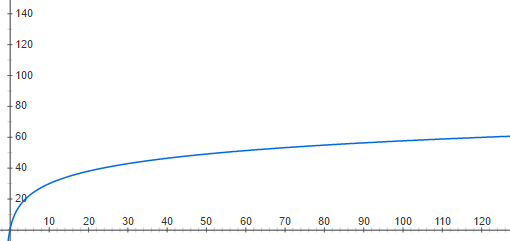
\includegraphics[scale=0.75]{images/bellicisme.png}
	\caption{�volution du bellicisme en fonction de la population}
	\label{fig:bellicisme}
\end{figure}

Nous avons choisi d'utiliser une fonction logarithmique pour �viter que les pays ne se fassent la guerre syst�matiquement lorsque leur population devient trop basse, �vitant ainsi de faire durer les guerres �ternellement.

\subsubsection{�v�nements}
\paragraph{Actions locales}
Au d�but de chaque "tour\footnote{Voir chapitre sur la Running Loop}", chaque peuple a une probabilit� donn�e (permettant un ajustement) de recevoir un �v�nement al�atoire influant sur ses attributs principaux. L'amplitude de l'�v�nement est elle aussi al�atoire (faible, moyen, fort) et en influencera les cons�quences. Par exemple l'�v�nement "Faible" Crise �conomique fera perdre des ressources au peuple impact�.
\paragraph{Actions globales}
Chaque "tour" il y a une probabilit� qu'un �v�nement affecte tous les peuples. Celui-ci agira sur l'attribut principal donn� de tous les peuples, par exemple l'�v�nement S�isme diminuera la population de chaque peuple d'une valeur comprise entre 1 et 3.
\paragraph{R�actions locales}
Chaque "tour", apr�s la r�solution des actions, chaque peuple aura une probabilit� (d�pendant des attributs du peuple) de d�clencher un �v�nement r�action, qui influera sur ses diff�rents attributs. Par exemple, si la richesse d'un peuple passe au dessus d'un certain seuil (ici 50), l'�v�nement Am�lioration de l'�ducation" pourra se d�clencher, augmentant ainsi l'�ducation du peuple.

\begin{figure}[H]
	\centering
		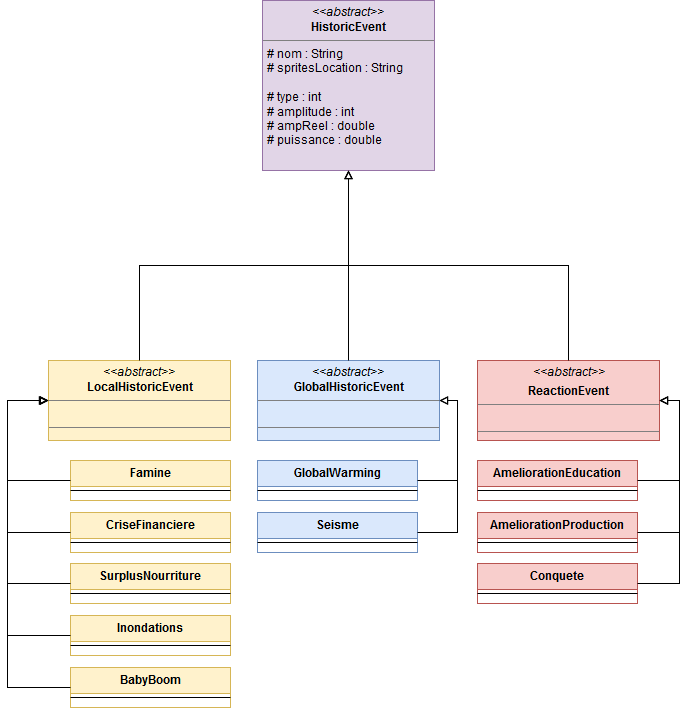
\includegraphics[scale=0.5]{images/eventUML.png}
	\caption{Diagramme UML des diff�rents �v�nements}
	\label{fig:events}
\end{figure}

\subsection{Classes fonctionnelles}
\subsubsection{Guerre et commerce}
Chaque tour, des guerres et des liens commerciaux commencent, ou non, entre les peuples, en fonction de leurs caract�ristiques secondaires. Ces relations n'influent que sur les attributs principaux.
\newline
La guerre est co�teuse en population et en richesses pour les deux peuples. Le commerce apporte un b�n�fice mutuel, mais plus un peuple dispose de puissance politique et plus il sera capable de tirer b�n�fice de ses liens commerciaux.
\newline
\newline
On �tudiera chaque bin�me de pays potentiel pour identifier lesquels ont les valeurs d'attributs n�cessaires pour entrer en guerre.
\newline
Un couple de peuple est "�ligible" � entrer en guerre si la somme de leurs bellicismes est sup�rieure ou �gale � un seuil fix� (ici 150).
\newline
Pour le commerce, il s'agit de la somme de leur attractivit� qui sera prise en compte, on �tudiera comme ci dessous pour �viter tout doublon.
\newline
\newline
\begin{center}
\begin{tabular}{|c|c|c|c|}
\hline
& Peuple 1 & Peuple 2 & Peuple 3 \\
\hline
Peuple 1 & X & Guerre / Commerce & Guerre / Commerce \\
\hline
Peuple 2 & X & X & Guerre / Commerce \\
\hline
Peuple 3 & X & X & X \\
\hline
\end{tabular}
\end{center}

Les cons�quences de la guerre sont ensuite r�solues, la population de chaque pays en guerre est diminu�e de la puissance militaire de leur adversaire multipli�e par un coefficient de r�duction, ici 0.01.
\newline
La guerre est trait�e avant le commerce, car dans notre syst�me deux pays en guerre ne peuvent pas commercer entre eux.

\subsubsection{Immigration et croissance}
Chaque "tour", les pays perdront ou gagneront de la population, proportionnellement � leur taux d'immigration (un taux positif signifie qu'un pays attire les migrants, tandis qu'une immigration n�gative poussera les habitants du pays en question � le quitter).
\newline
\newline
Une am�lioration possible serait une approche plus r�aliste en r�alisant un "pool" de population constitu� de toutes les populations quittant leurs pays de d�part. Cette masse de population serait r�partie en fonction du taux d'immigration positive de chaque pays et, s'il y  a des "exc�dents" par rapport � la demande, ceux-ci seraient attribu�s par rapport au pays de d�part.
\newline
La croissance est une augmentation fixe de la population de chaque pays � chaque tour, ici la croissance sera de 1 par tour.
\newline
\newline
L'immigration est g�r�e dynamiquement en fonction des besoins de chaque pays. Un pays ayant une une densit� de population n�gative\footnote{Se r�f�rer au calcul de la densit�.} verra sa population en trop "quitter" le pays et �tre affect�e � une "pool" de population qui sera r�partie sur les pays en demande de population, l'ordre de r�partition �tant al�atoire et changeant � chaque tour pour �viter que les premiers pays de la liste ne s'accaparent tous les flux migratoires.

\subsubsection{RunningLoop}
La Running loop, ou boucle de fonctionnement est l'�pine dorsale de la partie backend. Elle va g�rer l'ordre dans lequel seront effectu�s les diff�rents calculs li�s au guerres, commerces et �v�nements, selon le sch�ma ci-dessous.

\begin{figure}[H]
	\centering
		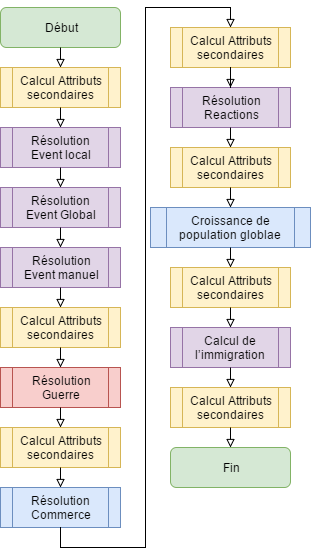
\includegraphics[scale=0.5]{images/RunningLoop.png}
	\caption{Sch�ma de fonctionnement de la RunningLoop}
	\label{fig:runningloop}
\end{figure}

�tant l'une des classes principales de la partie calcul et n'�tant instanci�e qu'une seule fois, c'est elle qui contiendra les diff�rents �l�ments statiques :
\begin{itemize}
\bulletitem{Logs de d�bugage}
\bulletitem{Logs � afficher � l'utilisateur}
\bulletitem{Nombre de cycles �coul�s}
\bulletitem{Liste d'�v�nements entr�s manuellement}
\end{itemize}
Cette classe impl�mente aussi les diff�rentes m�thodes pour ajouter du texte aux diff�rents logs.
\begin{figure}[H]
	\centering
		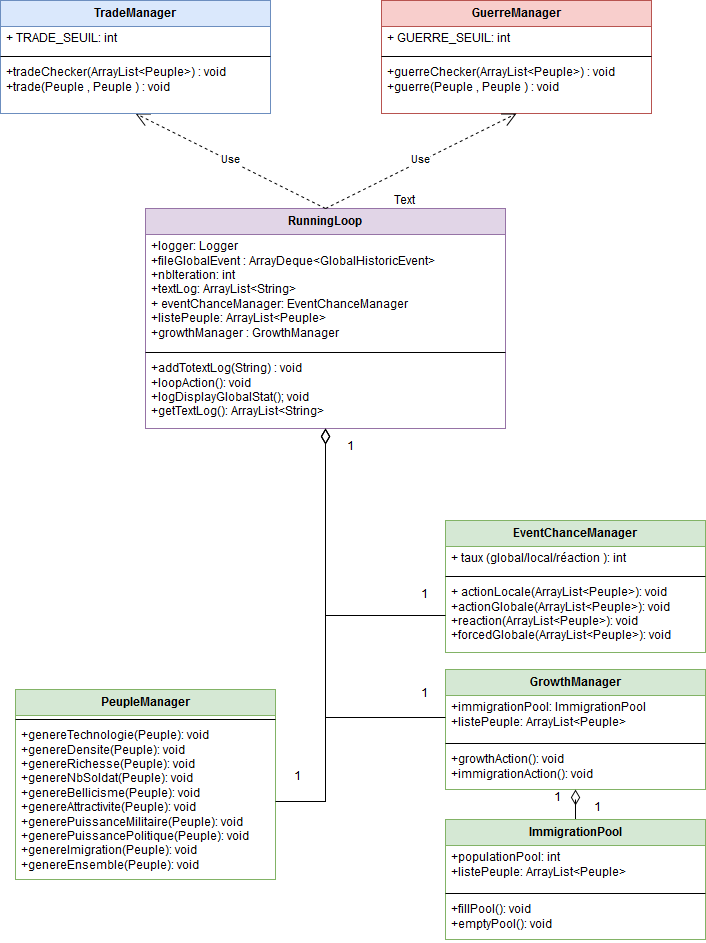
\includegraphics[scale=0.5]{images/RunningLoopUML.png}
	\caption{UML de la RunningLoop}
	\label{fig:runningloopuml}
\end{figure}

\subsubsection{Gestionnaire d'�v�nements}
Il existe un gestionnaire pour chaque type d'�v�nement (local, global, r�action). Ceux-ci instancient chacun une liste contenant tous les diff�rents �l�ments.
\newline
C'est dans ces classes que sont impl�ment�es les diff�rentes m�thodes d'action des �v�nements, tandis que les probabilit�s d'apparition des �v�nements sont g�r�es par la classe EventChanceManager. L'objectif �tait ici d'encapsuler chaque �l�ment de mani�re � rendre le programme le plus clair possible.
\begin{figure}[H]
	\centering
		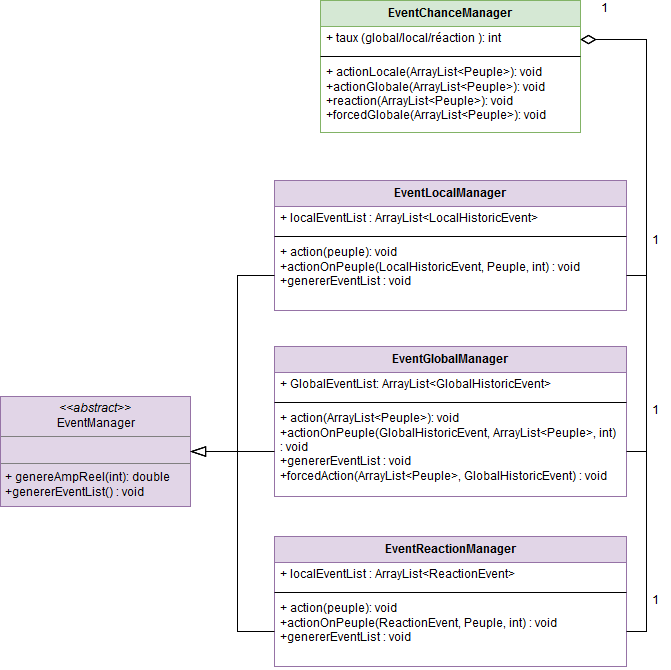
\includegraphics[scale=0.5]{images/managerUML.png}
	\caption{UML des diff�rents gestionnaires}
	\label{fig:manageruml}
\end{figure}

\subsection{Syst�mes de logs et de d�bogage}
\subsubsection{Log4J}
Durant les premi�res phases du d�veloppement, nous avons �t� confront�s � plusieurs probl�mes de d�bogage et d'�quilibrage dans les m�caniques mises en place.
\newline
Plut�t d'utiliser, comme nous le faisions pr�c�demment, de simples envois de cha�nes de caract�res sur le flux d'erreur standard, nous avons choisi de mettre en place et d'utiliser la librairie Log4J pour obtenir un syst�me de logs plus complet.
\newline
Cela nous a permis de mettre en forme les diff�rentes donn�es renvoy�es par le programme, de les hi�rarchiser et de pouvoir comprendre quand et comment certaines fonctionnalit�s pouvaient poser probl�me. Par exemple, ce syst�me nous a permis de r�soudre un bug faisant augmenter de mani�re exponentielle les ressources des diff�rents pays � partir d'un certain nombre de cycles.
\begin{figure}[H]
	\centering
		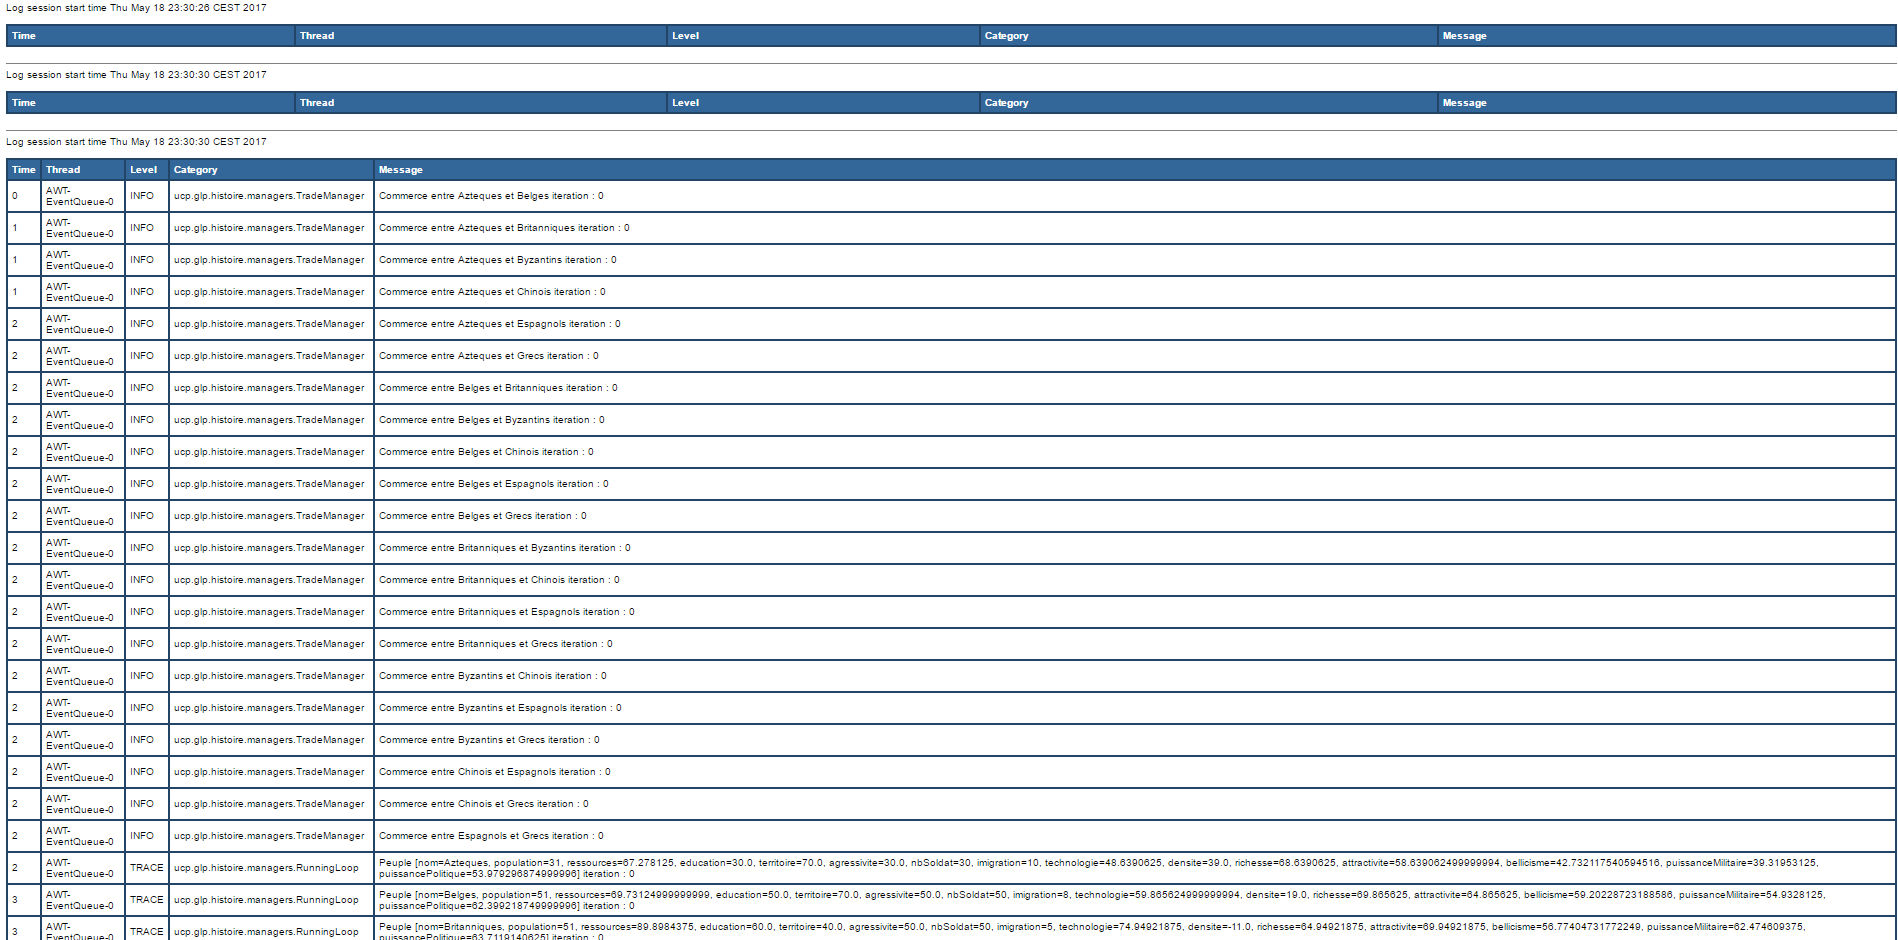
\includegraphics[scale=0.33]{images/logshtml.png}
	\caption{Aper�u des logs obtenus gr�ce � Log4J en HTML}
	\label{fig:logshtml}
\end{figure}

\subsubsection{JUnit}
Dans la m�me optique que pr�c�demment et pour aller un peu plus loin en automatisant les tests sur certaines des fonctions de notre moteur, nous avons choisi d'utiliser le framework JUnit.
\newline
Celui-ci nous a notamment �t� utile pour tester les diff�rentes �volutions des peuples au fil des tours, sur de tr�s grandes it�rations.
\clearpage
\section{Interface Utilisateur}
\label{sec:gui}

\subsection{Fen�tre}
La fen�tre du programme aura une taille pr�d�finie de 1280x720 pixels et n'est pas redimensionnable. Cette dimension a �t� choisir car elle correspond � une r�solution de 16:9 et est � la fois suffisamment petite pour ne pas d�border de la plupart des �crans, et suffisamment grande pour nous permettre d'afficher des �l�ments suffisamment d�taill�s.
\begin{figure}[H]
	\centering
		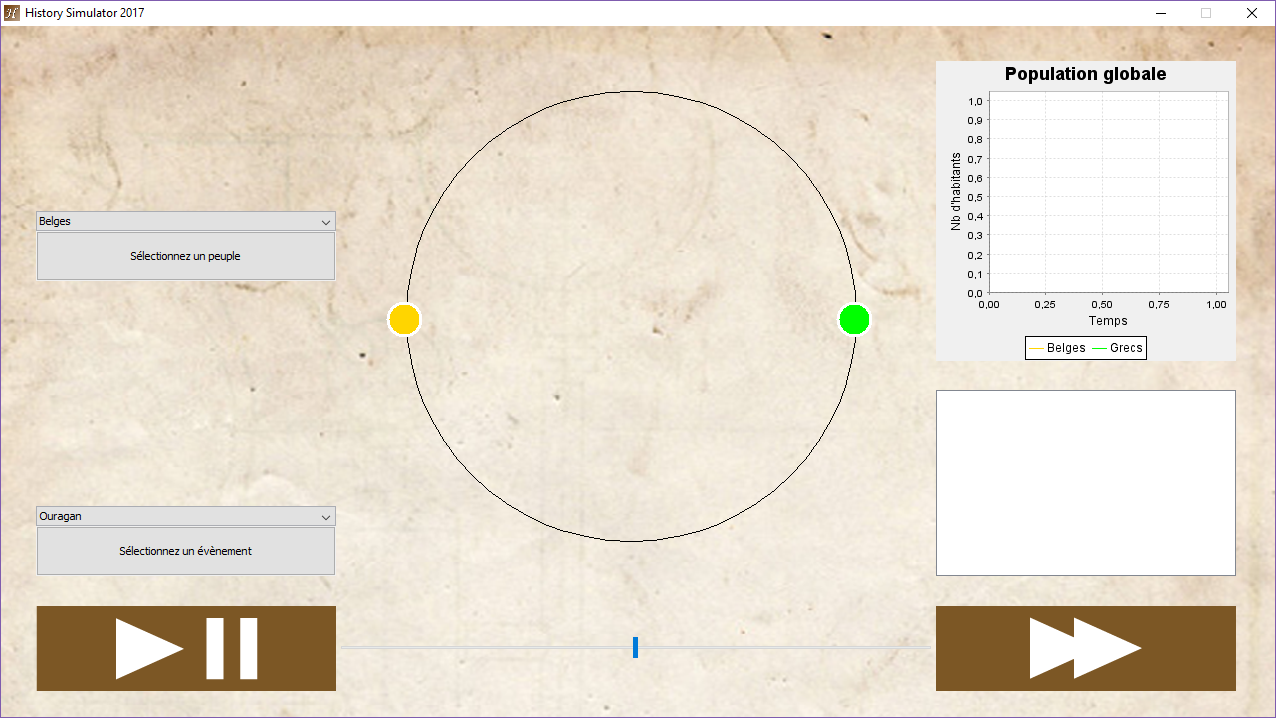
\includegraphics[scale=0.5]{images/window.png}
	\caption{Fen�tre}
	\label{fig:window}
\end{figure}

\subsection{�coulement du temps}
Dans la partie basse de l'interface, trois �l�ments permettent de g�rer le passage du temps. � gauche, un bouton permet de mettre en pause ou de reprendre le passage automatique des cycles. Au milieu, un curseur sert � r�gler la vitesse d'�coulement du temps lors des cycles automatiques. 
\newline
Enfin, � droite, un bouton permet de passer au cycle suivant manuellement, m�me si l'�coulement du temps est en pause.

\subsection{Statistiques centrales}
Au centre de la fen�tre, des statistiques sont affich�es. Par d�faut, il s'agira d'un diagramme repr�sentant les pays ainsi que leurs relations. Si un peuple est s�lectionn�\footnote{Voir plus bas pour la s�lection d'un peuple}, les statistiques affich�es seront celles du peuple en question, et plus de d�tails seront fournis sur celui-ci.
\begin{figure}[H]
	\centering
		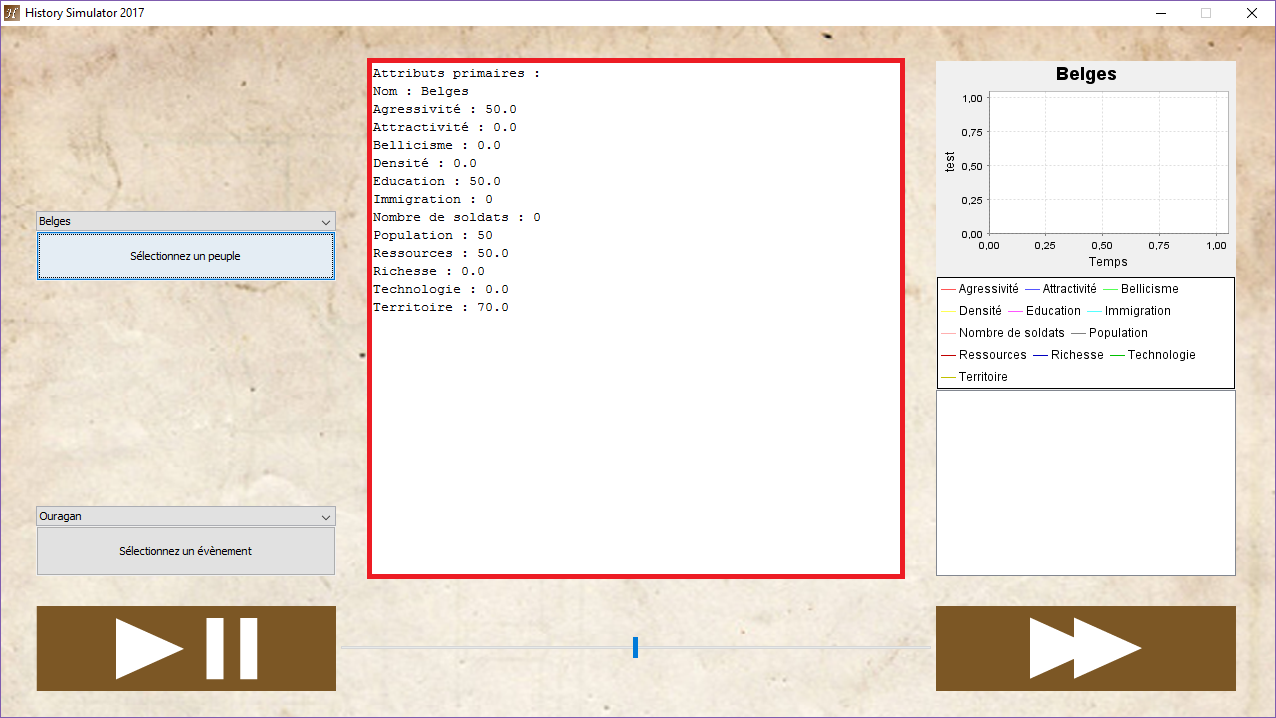
\includegraphics[scale=0.5]{images/details.png}
	\caption{D�tails}
	\label{fig:details}
\end{figure}

\subsection{S�lectionner un peuple}
Un menu d�roulant comportant tous les peuples et un bouton de validation sont � gauche de la fen�tre. Ceux-ci permettent de s�lectionner un peuple. En validant, on a acc�s � ses statistiques d�taill�es au centre de l'interface.
\newline
Il y a �galement une option \textit{Aucun} permettant de revenir � l'affichage des statistiques globales des relations entre les peuples.

\subsection{S�lectionner un �v�nement}
Les �v�nements peuvent �tre d�clench�s manuellement par l'utilisateur, via un menu d�roulant et un bouton de validation. Il est �galement possible de param�trer la puissance de l'�v�nement, ainsi que de d�sactiver les �v�nements al�atoires.
\newline
Si un peuple est s�lectionn�, l'�v�nement le concernera. Sinon, le menu d�roulant n'affichera que les �v�nements d'ampleur globale.
\subsection{Compte-rendu des �v�nements}
� droite de l'interface, une zone de texte liste tous les �v�nements s'�tant produits au cours du dernier cycle.
\clearpage
\section{Conclusion}
\label{sec:conclusion}

\noindent Au terme de ce projet, nous avons beaucoup appris et sommes fiers du programme final.
\newline
N�anmoins, celui-ci est loin d'�tre parfait, et plusieurs am�liorations seraient encore possibles.
\newline
Il serait par exemple possible de permettre � l'utilisateur de cr�er lui-m�me les peuples qu'il souhaite voir en jeu, ou le th�me qu'il souhaite utiliser.
\newline
L'�quilibrage n'est lui non plus pas parfait, et il serait int�ressant de cr�er un syst�me d'�quilibrage automatique en fonction des r�sultats des derni�res simulations.
\newline
\newline
Toutefois, nous sommes parvenus � nous organiser correctement de mani�re � ce que l'interface utilisateur et le moteur avancent de mani�re parall�le et synchronis�e. Les objectifs ont �t� r�alis�s dans les d�lais que nous avions convenu et nous avons tous deux consolid� nos connaissances g�n�rales et nos m�thodes de travail.

%Une section "remerciements" pourrait �tre int�ressante. C'est une section non num�rot� (avec un * )
\section*{Remerciements}
Merci � notre professeur r�f�rent T. Liu pour son accompagnement, ses conseils et ses encouragements tout au long de ce projet. Gr�ce � sa p�dagogie et sa confiance en nos capacit�s, il nous a permis de donner le meilleur de nous-m�me pendant ce semestre.

%R�f�rences bibliographiques du document
%\bibliographystyle{plain}
%\bibliography{bibliographies}
%\nocite{*}

\end{document}
